\section{Large Figures}\label{sec:app}

\subsection{Schematic of sensorboard}\label{app:schemmain}
%Image of schematic(s) (Rev 3)
\begin{figure}[h]
	\centering
    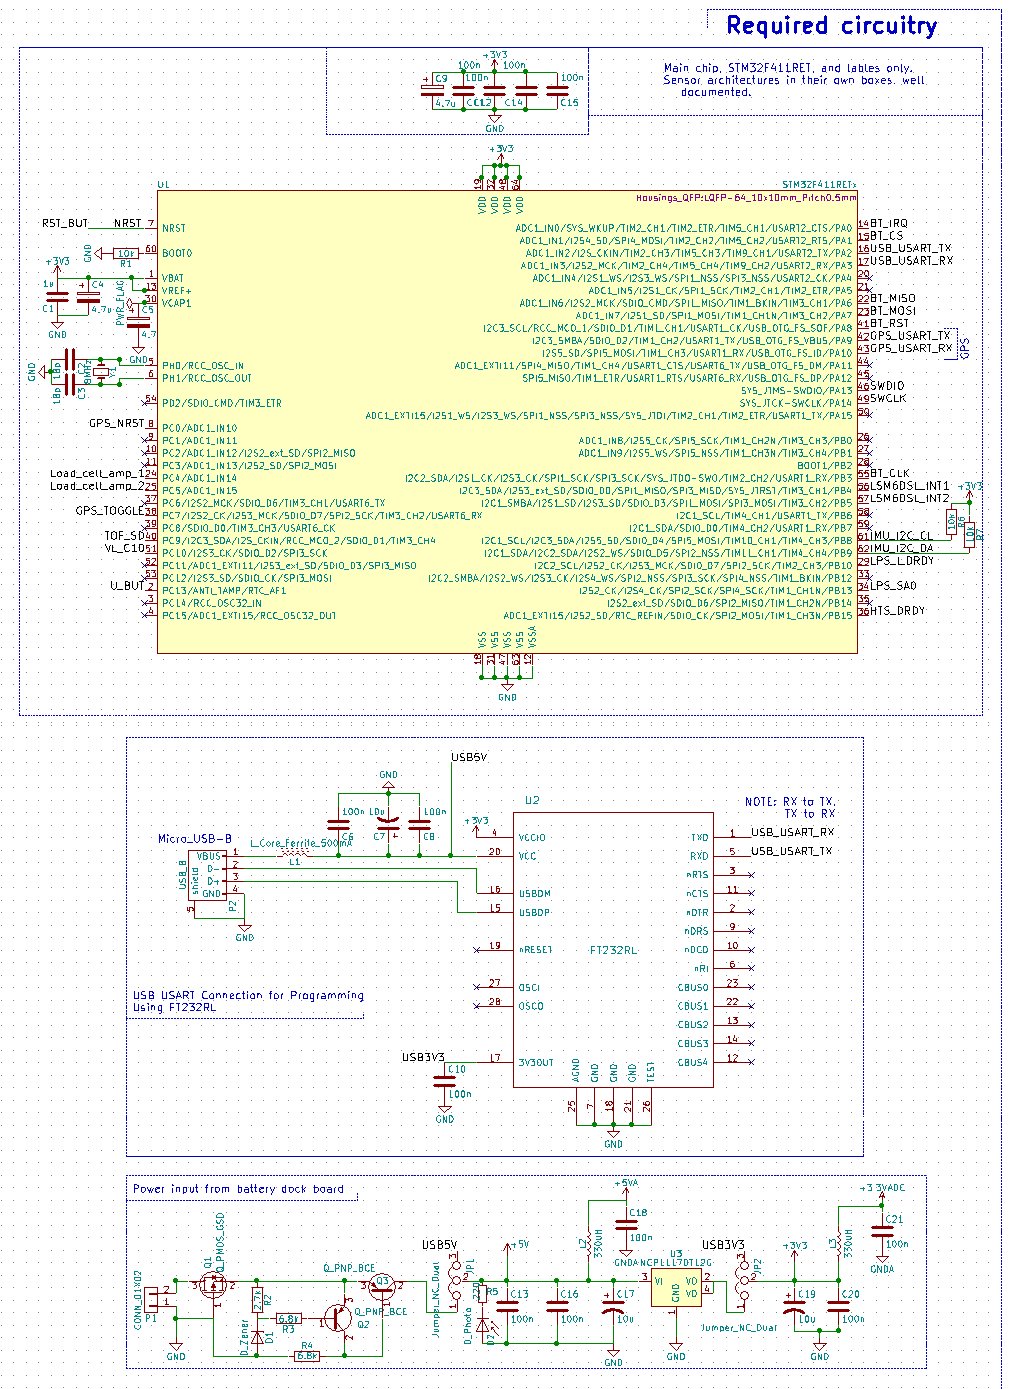
\includegraphics[width=.93\linewidth]{Figures/schem_r3_a.png}
	\caption{Schematic of revision 3, part a: Required circuitry.}
	\label{fig:schr3a}
\end{figure}
\begin{figure}[h]
	\centering
    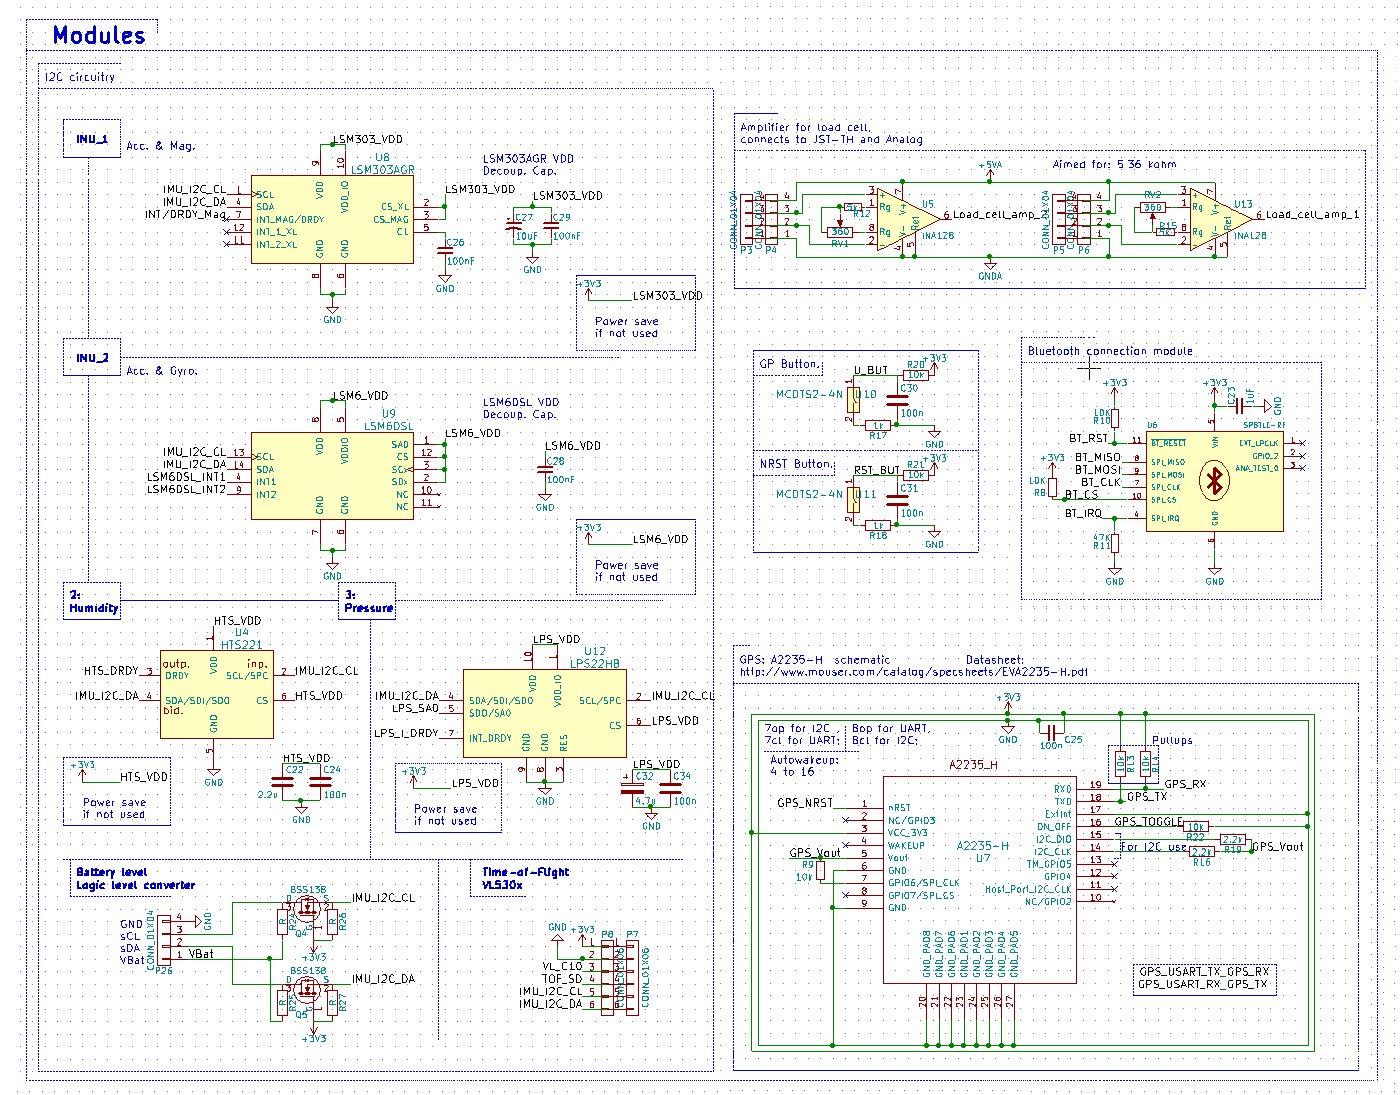
\includegraphics[width=\linewidth]{Figures/schem_r3_b.png}
	\caption{Schematic of revision 3, part b: Modules.}
	\label{fig:schr3b}
\end{figure}
\begin{figure}[h]
	\centering
    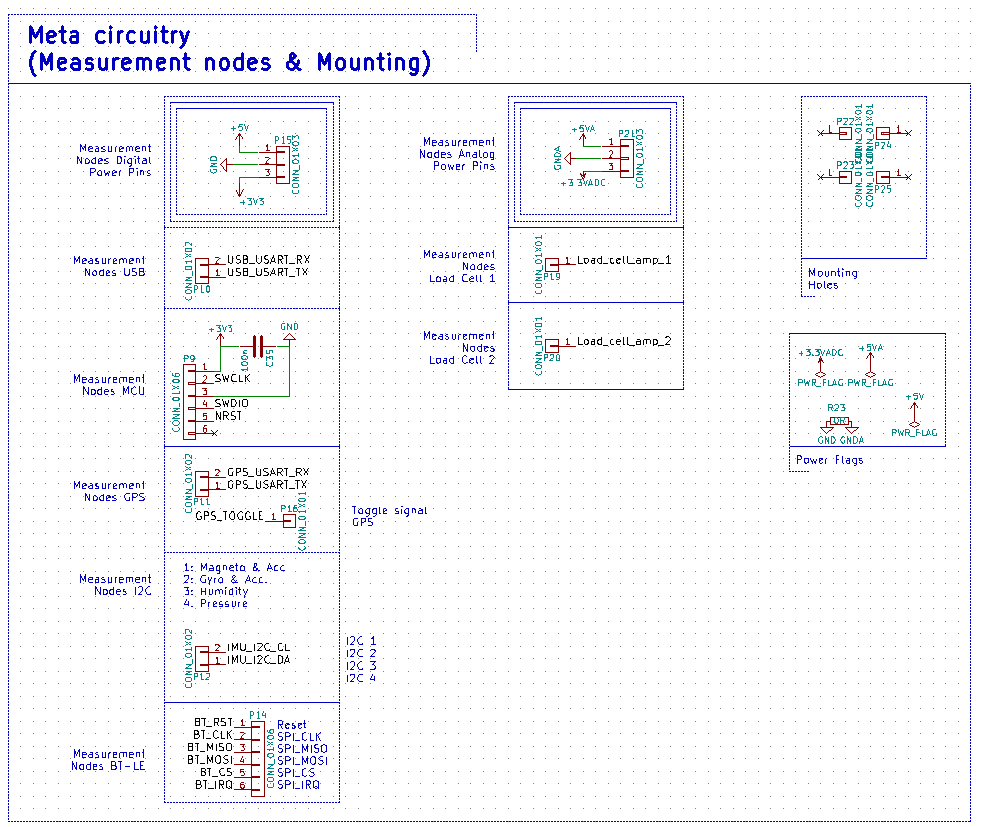
\includegraphics[width=\linewidth]{Figures/schem_r3_c.png}
	\caption{Schematic of revision 3, part c: Meta circuitry.}
	\label{fig:schr3c}
\end{figure}

\clearpage
\subsection{Schematic of \gls{bms}}\label{app:bms}
\begin{figure}[h]
	\centering
    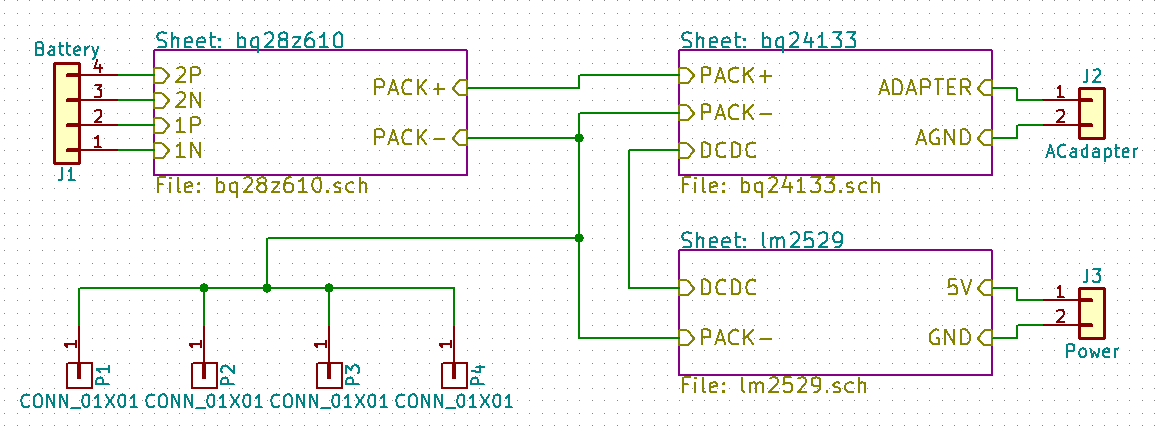
\includegraphics[width=.9\linewidth]{Figures/gasgauge_sch_root.png}
	\caption{Root schematic of \gls{bms} circuitry.}
	\label{fig:schbmsr}
\end{figure}
\begin{figure}[h]
	\centering
    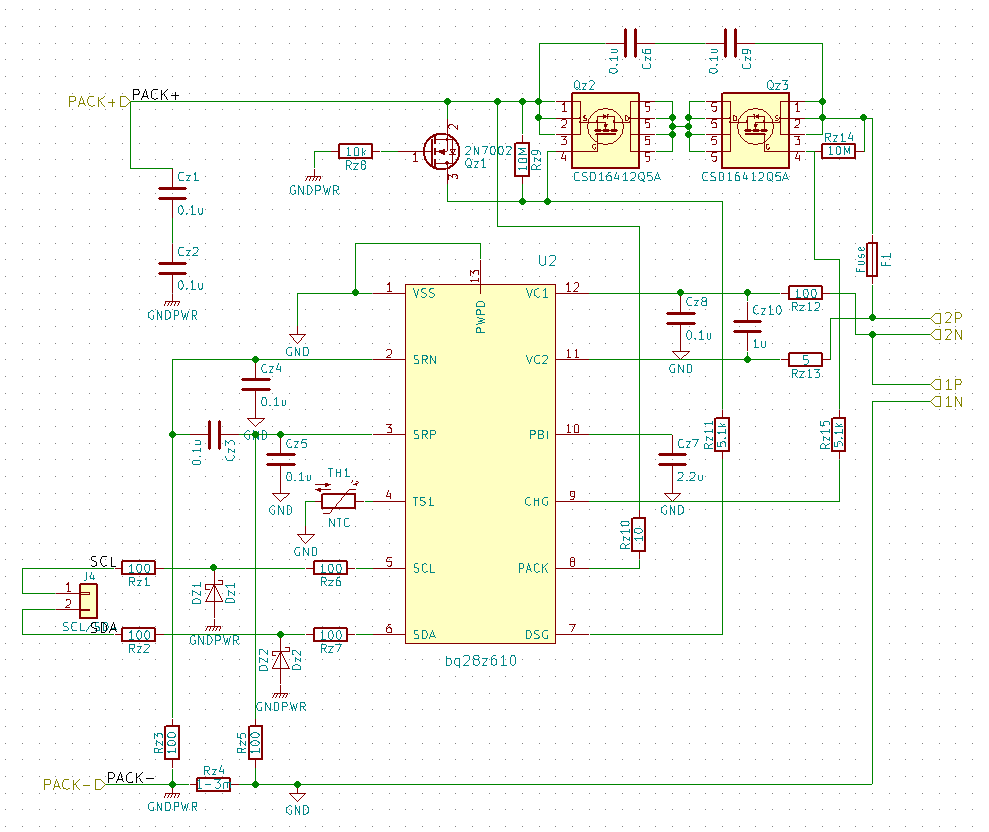
\includegraphics[width=.9\linewidth]{Figures/gasgauge_sch_bq28z610.png}
	\caption{Schematic of \gls{bms}, part a: bq28z610.}
	\label{fig:schbmsr}
\end{figure}
\begin{figure}[h]
	\centering
    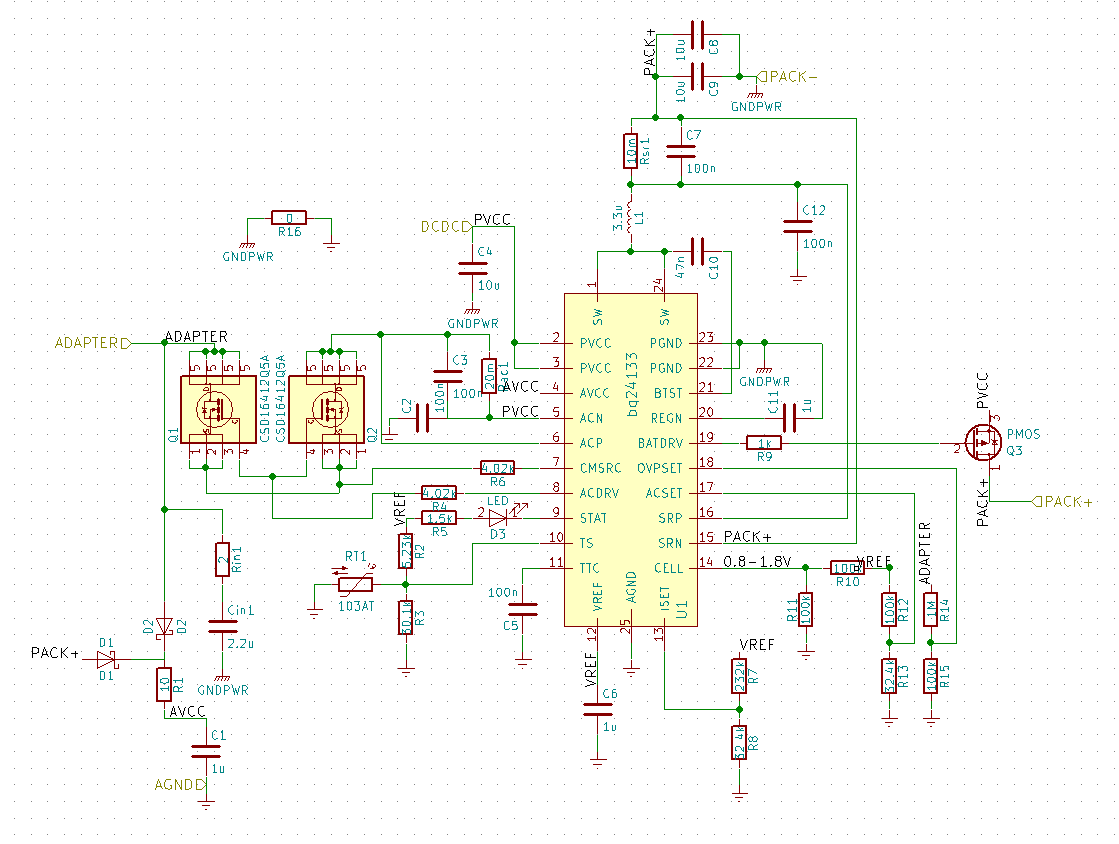
\includegraphics[width=\linewidth]{Figures/gasgauge_sch_bq24133.png}
	\caption{Schematic of \gls{bms}, part b: bq24133.}
	\label{fig:schbmsr}
\end{figure}
\begin{figure}[h]
	\centering
    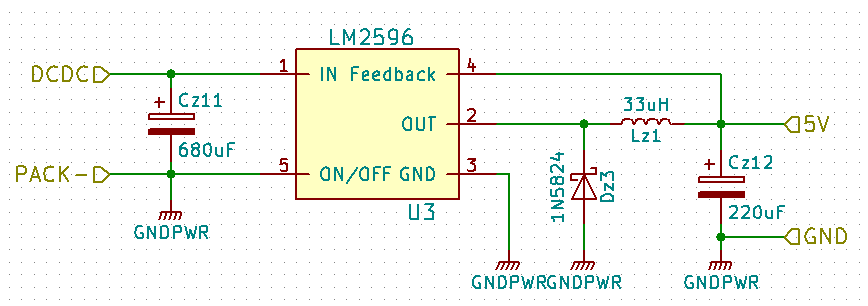
\includegraphics[width=\linewidth]{Figures/gasgauge_sch_lm2529.png}
	\caption{Schematic of \gls{bms}, part c: lm2596.}
	\label{fig:schbmsr}
\end{figure}


\clearpage
\subsection{CubeMX software}\label{sec:app:mxc}
% Image of CubeMX software
\begin{figure}[tbh]
	\centering
    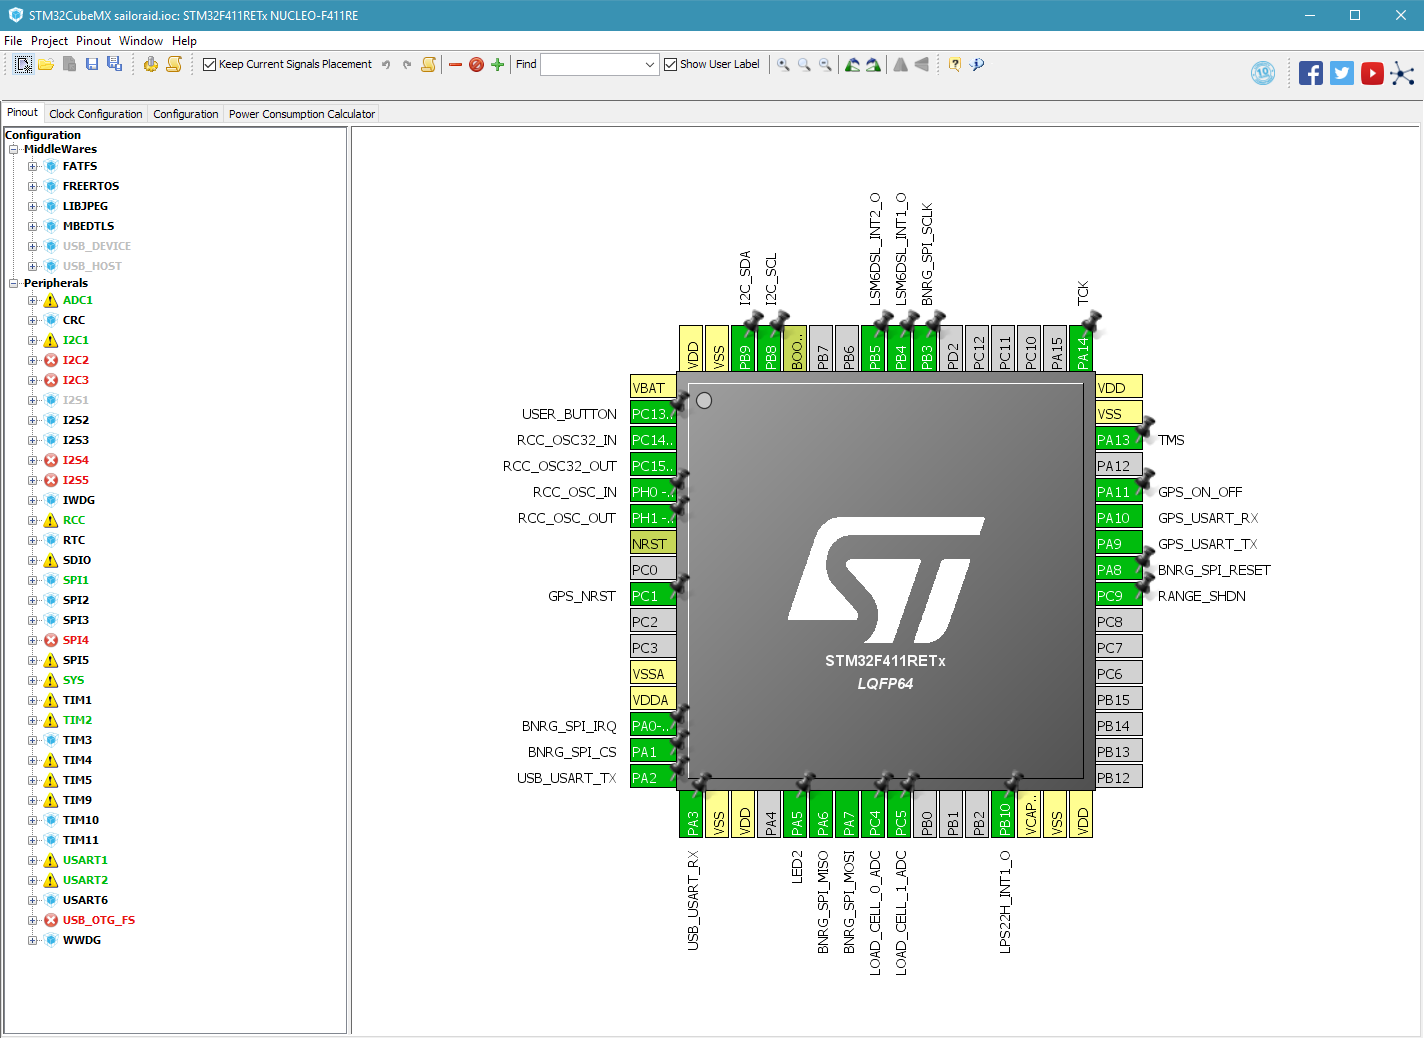
\includegraphics[width=\linewidth]{Figures/MXCube.png}
	\caption{CubeMX software}
	\label{fig:mxc}
\end{figure}

\clearpage
\section{Other Figures}
\subsection{Casing Dimensions}
\begin{figure}[htb]
	\centering
    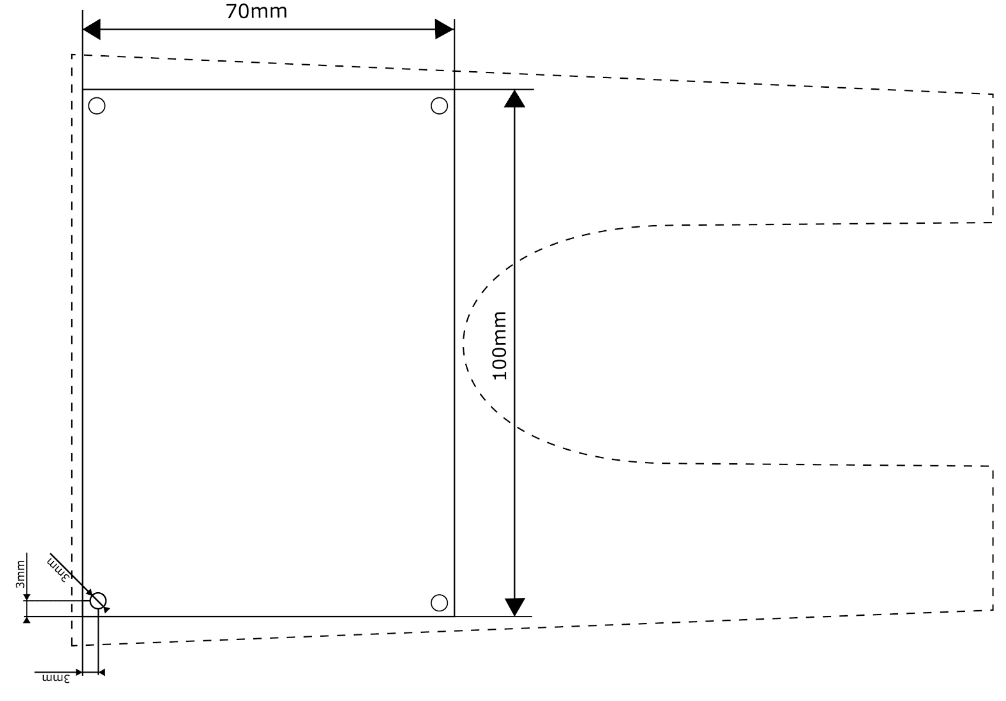
\includegraphics[width=\linewidth]{Figures/casing_dimensions.png}
	\caption{System enclosure shape and dimensions}
	\label{fig:casdim}
\end{figure}
%Image of circuit board(s) are sectionlocals labled as "fig:pcbr*"

%Local. Image of casing

%INSERT Image of complete/mounted system
